\documentclass{beamer}
\usetheme{metropolis}
\usepackage{graphicx}
\usepackage{subfig}
\usepackage{tcolorbox}
\usepackage{mathtools}
\title{Computer Logic and Digital Circuit Design (PHYS306/COSC330): Unit 2.3}
\author{Jordan Hanson}
\institute{Whittier College Department of Physics and Astronomy}

\begin{document}
\maketitle

\section{Summary}

\begin{frame}{Unit 2.3 Summary - Theoretical Logic Gates, and Operations}
\textbf{Reading: DF Chapter 3-4 (Moodle)}
\begin{enumerate}
\item Logic Gates
\begin{itemize}
\item Circuit diagram
\item Truth table
\item Timing diagram
\item Boolean logic
\end{itemize}
\item \alert{Boolean algebra I}
\item IC Circuits, \textbf{data sheets}
\item \alert{Boolean algebra II}
\end{enumerate}
\textbf{Homework: Chapter 3, ex. 1-22 (two weeks)}
\end{frame}

\section{Boolean Algebra Basics}

\begin{frame}{Boolean Algebra Basics}
\textbf{Good paper topic}: George Boole and Claude Shannon in the mid-19th century, early 20th century. \\ \vspace{0.5cm}
\textbf{\alert{Boolean}} or logical algebra - \textit{An Investigation of the Laws of Throught, on Which Are Founded the Mathematical Theories of Logic and Probabilities} (Boole's title) \\ \hrulefill \\
\textbf{What does \textit{an algebra} contain?}
\begin{enumerate}
\item Variables or \textit{literals}
\item \textit{complements} (resembles \textit{identities, reciprocals, and nulls})
\item Sums are ORs
\item Products are ANDs
\end{enumerate}
\end{frame}

\begin{frame}{Boolean Algebra Basics}
\small
An algebra has many objects, properties, and rules.  An extensive list is outside our scope.  \\ \vspace{0.1cm}
\textbf{Boolean or logical algebra} has these \textit{objects}: \\ \vspace{0.1cm}
\begin{enumerate}
\item Variables: $A$ is a variable, either TRUE or FALSE
\item complements: $\overline{A}$ is the \textit{complement} of $A$, inverting the input \\ \vspace{0.1cm}
\end{enumerate}
\begin{figure}
\centering
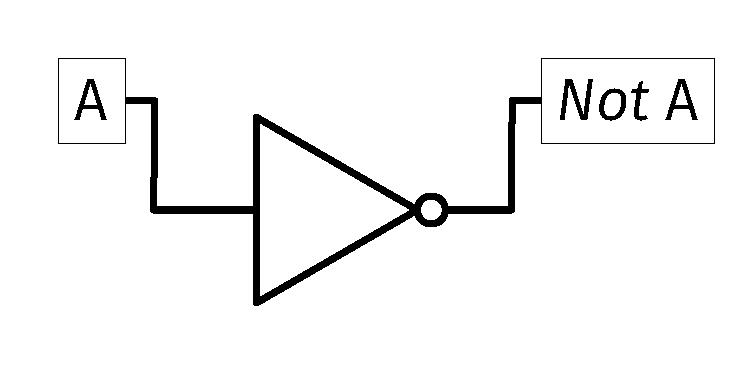
\includegraphics[width=0.5\textwidth]{figures/NOTOperation.pdf}
\caption{\label{fig:NOT} The inverter performs the complement operation at gate-level, $\overline{A} = NOT~A$.}
\end{figure}
\end{frame}

\begin{frame}{Boolean Algebra Basics}
\small
\textit{AND is multiplication, and OR is addition.  Refer to Chapter 2 DF.} \\ \vspace{0.1cm}
\textbf{Boolean or logical algebra} has these \textit{properties}:
\begin{enumerate}
\item \alert{Property of commutativity}
\begin{itemize}
\item \textbf{Addition version: $A + B = B + A$}
\item (\textit{an OR gate does not distinguish between inputs})
\item \textbf{Mutliplication version: $AB = BA$}
\item (\textit{an AND gate does not distinguish between inputs})
\end{itemize}
\item \alert{Property of Associativity}
\begin{itemize}
\item \textbf{Addition version: $(A+B)+C = A+(B+C)$}
\item \textit{OR gate order does not matter}.
\item \textbf{Mutliplication version: $(AB)C = A(BC)$}
\item \textit{AND gate order does not matter}.
\end{itemize}
\item \alert{Property of Distribution}
\begin{itemize}
\item $A(B+C) = AB+BC$ (\textit{gate input and gate order})
\end{itemize}
\end{enumerate}
\end{frame}

\begin{frame}{Boolean Algebra Basics}
\small
\begin{columns}[T]
\begin{column}{0.5\textwidth}
\textbf{Boolean or logical algebra} has these \textit{rules}:
\begin{enumerate}
\item $A+0 = A$
\item $A+1=1$
\item $A\cdot 0=0$
\item $A\cdot 1=A$
\item $A+A=A$
\item $A+\overline{A}=1$
\item $AA = A$
\item $A\overline{A}=0$
\item $\overline{\overline{A}} = A$
\end{enumerate}
\end{column}
\begin{column}{0.5\textwidth}
\textbf{Boolean or logical algebra} has these \textit{special rules}:
\begin{enumerate}
\item $A+AB = A$
\item $A+\overline{A}B=A+B$
\item $(A+B)(A+C) = A+BC$
\end{enumerate} \vspace{0.2cm}
\tiny
\textbf{Exercises:} \\ \hrulefill
\begin{itemize}
\item Prove special rule (1) with a truth table
\item Why is special rule (1) intuitive?
\item Prove special rule (2) with a truth table
\item Why is special rule (2) intuitive?
\item \textbf{Group board exercise:} Prove special rule (3) \textit{Hint: this requires rules 2, 4, and 7.  This is good practice at \textbf{gate simplification.}}
\end{itemize}
\end{column}
\end{columns}
\end{frame}

\begin{frame}{Boolean Algebra Basics}
\begin{columns}[T]
\begin{column}{0.5\textwidth}
De Morgan's Theorems \\ \hrulefill
\begin{itemize}
\small
\item \textbf{First theorem}: The complement of a product of literals is equal to the sum of the complements of the literals.
\item \textbf{Second theorem}: The complement of a sum of literals is equal to the product of the complements of the literals.
\end{itemize}
\end{column}
\begin{column}{0.5\textwidth}
\begin{itemize}
\item First theorem: $\overline{AB} = \overline{A}+\overline{B}$
\item Second theorem: $\overline{A+B} = \overline{A}\overline{B}$
\end{itemize} \hrulefill \\
For example: \\ 
$\overline{(AB+BC)} = \overline{AB}~\overline{BC} = (\overline{A}+\overline{B})(\overline{B}+\overline{C})$
\end{column}
\end{columns}
\end{frame}

\begin{frame}{Boolean Algebra Basics}
\small
\textbf{Group board exercise}: Show that
\begin{equation}
\begin{multlined}
\boxed{
\overline{(A+B)(B+C)}+\overline{(A+\overline{A}B)(B+\overline{B}A)}=\overline{A}+\overline{B}+\overline{C}} \label{eq:prob1}
\end{multlined}
\end{equation}
\begin{itemize}
\item \textit{Hint}: use De Morgan's two theorems
\item \textit{Hint}: use special rule 3
\item \textit{Hint}: consider the regular rules
\end{itemize}
\textbf{Group board exercise}: Create a circuit using logic gates that represents the left-hand side of Eq. \ref{eq:prob1}, and do the same for the right-hand side.  How many gates fewer are there in the right-hand solution?
\end{frame}

\begin{frame}{Boolean Algebra Basics}
\small
\textbf{Group board exercise}: Show that
\begin{equation}
\boxed{
\begin{multlined}
(AB+C(B+A))+\overline{(AB+C(B+A))}(AC+B(C+A)) \\ = AB+AC+BC \label{eq:prob2}
\end{multlined}}
\end{equation}
\begin{itemize}
\item \textit{Hint}: use special rule 2
\item \textit{Hint}: use De Morgan's two theorems
\end{itemize}
\textbf{Group board exercise}: Create a circuit using logic gates that represents the left-hand side of Eq. \ref{eq:prob2}, and do the same for the right-hand side.  How many gates fewer are there in the right-hand solution?
\end{frame}

\section{Conclusion}

\begin{frame}{Unit 2.3 Summary - Theoretical Logic Gates, and Operations}
\textbf{Reading: DF Chapter 3-4 (Moodle)}
\begin{enumerate}
\item Logic Gates
\begin{itemize}
\item Circuit diagram
\item Truth table
\item Timing diagram
\item Boolean logic
\end{itemize}
\item \alert{Boolean algebra I}
\item IC Circuits, \textbf{data sheets}
\item \alert{Boolean algebra II}
\end{enumerate}
\textbf{Homework: Chapter 3, ex. 1-22 (two weeks)}
\end{frame}

\end{document}
